%--------------------------------------
%ELECTROTECHNIQUE - SCHEMA DE LIAISON A LA TERRE
%--------------------------------------

%utiliser les environnement \begin{comment} \end{comment} pour mettre en commentaire le préambule une fois la programmation appelée dans le document maître (!ne pas oublier de mettre en commentaire \end{document}!)

\begin{comment}

\documentclass[a4paper, 11pt, twoside, fleqn]{memoir}

\usepackage{AOCDTF}

\marqueurchapitre

% lien éditeur : https://www.mathcha.io/editor/MX589f23ULmHBnmM8pFwj7EL1tYdMv57HwxB39K

%--------------------------------------
%corps du document
%--------------------------------------

\begin{document} %corps du document
	\openleft %début de chapitre à gauche

\end{comment}

\begin{figure}[H]
\caption{Boucle à fond de fouille}



\tikzset{every picture/.style={line width=0.75pt}} %set default line width to 0.75pt        

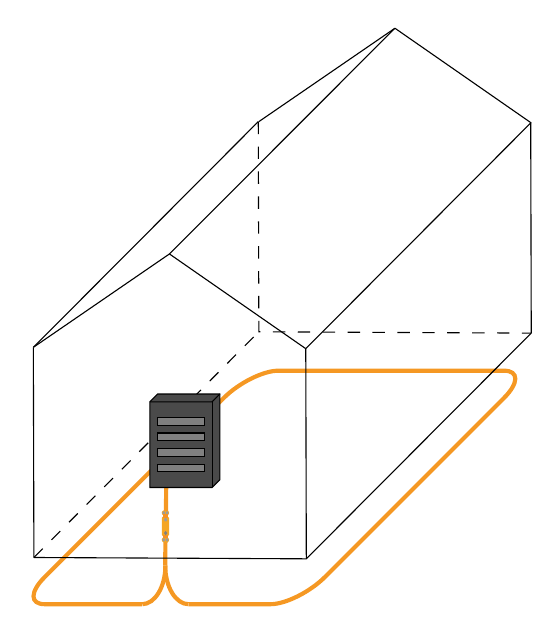
\begin{tikzpicture}[x=0.75pt,y=0.75pt,yscale=-0.75,xscale=0.75]
%uncomment if require: \path (0,481); %set diagram left start at 0, and has height of 481

%Straight Lines [id:da30799843530611115] 
\draw [color={rgb, 255:red, 245; green, 152; blue, 35 }  ,draw opacity=1 ][line width=1.5]    (240,360) -- (239.84,375.16) ;
%Straight Lines [id:da5305354409070833] 
\draw  [dash pattern={on 4.5pt off 4.5pt}]  (299.65,90) -- (300,225) -- (475,225.85) ;
%Straight Lines [id:da20935901156494685] 
\draw  [dash pattern={on 4.5pt off 4.5pt}]  (155.5,370) -- (300,225) ;
%Straight Lines [id:da9663799350386381] 
\draw    (155.15,235) -- (155.5,370) ;
%Straight Lines [id:da6956273497313757] 
\draw    (474.65,90.85) -- (475,225.85) ;
%Straight Lines [id:da46520744988670826] 
\draw    (155.15,235) -- (299.65,90) ;
%Straight Lines [id:da18568330552579893] 
\draw    (242.57,175) -- (330.15,235.85) ;
%Straight Lines [id:da08951823691400396] 
\draw    (155.15,235) -- (242.57,175) ;
%Straight Lines [id:da3765980997616395] 
\draw    (387.43,30) -- (475,90.85) ;
%Straight Lines [id:da20425329876761578] 
\draw    (300,90) -- (387.43,30) ;
%Straight Lines [id:da3978892908876972] 
\draw    (387.43,30) -- (242.57,175) ;
%Straight Lines [id:da3001438899283537] 
\draw    (474.65,90.85) -- (330.15,235.85) ;
%Rounded Rect [id:dp877203358644785] 
\draw  [color={rgb, 255:red, 245; green, 152; blue, 35 }  ,draw opacity=1 ][line width=1.5]  (277.5,267.5) .. controls (287.16,257.84) and (302.84,250) .. (312.5,250) -- (457.5,250) .. controls (467.16,250) and (467.16,257.84) .. (457.5,267.5) -- (342.5,382.5) .. controls (332.84,392.16) and (317.16,400) .. (307.5,400) -- (162.5,400) .. controls (152.84,400) and (152.84,392.16) .. (162.5,382.5) -- cycle ;
%Straight Lines [id:da4856516771678496] 
\draw    (330.15,235.85) -- (330.5,370.85) ;
%Straight Lines [id:da20084021876297198] 
\draw    (155.5,370) -- (330.5,370.85) -- (475,225.85) ;
%Straight Lines [id:da14498872282205144] 
\draw [color={rgb, 255:red, 255; green, 255; blue, 255 }  ,draw opacity=1 ][line width=3]    (225.15,400) -- (254.97,400) ;
%Shape: Arc [id:dp8164801831387742] 
\draw  [draw opacity=0][line width=1.5]  (254.97,400) .. controls (254.93,400) and (254.89,400) .. (254.84,400) .. controls (246.59,400) and (239.9,388.89) .. (239.84,375.16) -- (254.84,375) -- cycle ; \draw  [color={rgb, 255:red, 245; green, 152; blue, 35 }  ,draw opacity=1 ][line width=1.5]  (254.97,400) .. controls (254.93,400) and (254.89,400) .. (254.84,400) .. controls (246.59,400) and (239.9,388.89) .. (239.84,375.16) ;
%Shape: Arc [id:dp4891672557856719] 
\draw  [draw opacity=0][line width=1.5]  (240,375.38) .. controls (239.88,388.93) and (233.29,399.86) .. (225.15,400) -- (225,375) -- cycle ; \draw  [color={rgb, 255:red, 245; green, 152; blue, 35 }  ,draw opacity=1 ][line width=1.5]  (240,375.38) .. controls (239.88,388.93) and (233.29,399.86) .. (225.15,400) ;
%Rounded Rect [id:dp13850405546686684] 
\draw  [color={rgb, 255:red, 245; green, 166; blue, 35 }  ,draw opacity=1 ][fill={rgb, 255:red, 245; green, 166; blue, 35 }  ,fill opacity=1 ] (238,341.33) .. controls (238,340.6) and (238.6,340) .. (239.33,340) -- (240.67,340) .. controls (241.4,340) and (242,340.6) .. (242,341.33) -- (242,341.33) .. controls (242,342.07) and (241.4,342.67) .. (240.67,342.67) -- (239.33,342.67) .. controls (238.6,342.67) and (238,342.07) .. (238,341.33) -- cycle ;
%Shape: Polygon [id:dp012352628803113719] 
\draw  [color={rgb, 255:red, 155; green, 155; blue, 155 }  ,draw opacity=1 ][fill={rgb, 255:red, 155; green, 155; blue, 155 }  ,fill opacity=1 ] (241.6,341.33) -- (241.35,341.91) -- (240.85,341.91) -- (240.6,341.33) -- (240.85,340.76) -- (241.35,340.76) -- cycle ;
%Shape: Polygon [id:dp617840417972505] 
\draw  [color={rgb, 255:red, 155; green, 155; blue, 155 }  ,draw opacity=1 ][fill={rgb, 255:red, 155; green, 155; blue, 155 }  ,fill opacity=1 ] (239.4,341.33) -- (239.15,341.91) -- (238.65,341.91) -- (238.4,341.33) -- (238.65,340.76) -- (239.15,340.76) -- cycle ;

%Rounded Rect [id:dp29263936410769587] 
\draw  [color={rgb, 255:red, 245; green, 166; blue, 35 }  ,draw opacity=1 ][fill={rgb, 255:red, 245; green, 166; blue, 35 }  ,fill opacity=1 ] (238,358.67) .. controls (238,357.93) and (238.6,357.33) .. (239.33,357.33) -- (240.67,357.33) .. controls (241.4,357.33) and (242,357.93) .. (242,358.67) -- (242,358.67) .. controls (242,359.4) and (241.4,360) .. (240.67,360) -- (239.33,360) .. controls (238.6,360) and (238,359.4) .. (238,358.67) -- cycle ;
%Shape: Polygon [id:dp39786342275295183] 
\draw  [color={rgb, 255:red, 155; green, 155; blue, 155 }  ,draw opacity=1 ][fill={rgb, 255:red, 155; green, 155; blue, 155 }  ,fill opacity=1 ] (241.6,358.67) -- (241.35,359.24) -- (240.85,359.24) -- (240.6,358.67) -- (240.85,358.09) -- (241.35,358.09) -- cycle ;
%Shape: Polygon [id:dp030526214760367876] 
\draw  [color={rgb, 255:red, 155; green, 155; blue, 155 }  ,draw opacity=1 ][fill={rgb, 255:red, 155; green, 155; blue, 155 }  ,fill opacity=1 ] (239.4,358.67) -- (239.15,359.24) -- (238.65,359.24) -- (238.4,358.67) -- (238.65,358.09) -- (239.15,358.09) -- cycle ;

%Rounded Rect [id:dp9275012189629497] 
\draw  [color={rgb, 255:red, 245; green, 166; blue, 35 }  ,draw opacity=1 ][fill={rgb, 255:red, 245; green, 166; blue, 35 }  ,fill opacity=1 ] (238,344.73) .. controls (238,344.33) and (238.33,344) .. (238.73,344) -- (241.27,344) .. controls (241.67,344) and (242,344.33) .. (242,344.73) -- (242,355.27) .. controls (242,355.67) and (241.67,356) .. (241.27,356) -- (238.73,356) .. controls (238.33,356) and (238,355.67) .. (238,355.27) -- cycle ;
%Shape: Polygon [id:dp7623761074716651] 
\draw  [color={rgb, 255:red, 155; green, 155; blue, 155 }  ,draw opacity=1 ][fill={rgb, 255:red, 155; green, 155; blue, 155 }  ,fill opacity=1 ] (240.69,345.73) -- (240.4,346.39) -- (239.83,346.39) -- (239.54,345.73) -- (239.83,345.07) -- (240.4,345.07) -- cycle ;
%Shape: Rectangle [id:dp25144871820084] 
\draw  [color={rgb, 255:red, 245; green, 145; blue, 35 }  ,draw opacity=1 ][fill={rgb, 255:red, 245; green, 145; blue, 35 }  ,fill opacity=1 ] (241,356) -- (239,356) -- (239,357.33) -- (241,357.33) -- cycle ;
%Shape: Rectangle [id:dp07880374452402983] 
\draw  [color={rgb, 255:red, 245; green, 145; blue, 35 }  ,draw opacity=1 ][fill={rgb, 255:red, 245; green, 145; blue, 35 }  ,fill opacity=1 ] (241,342.67) -- (239,342.67) -- (239,344) -- (241,344) -- cycle ;
%Shape: Ellipse [id:dp8682429169918172] 
\draw  [color={rgb, 255:red, 128; green, 128; blue, 128 }  ,draw opacity=1 ][fill={rgb, 255:red, 128; green, 128; blue, 128 }  ,fill opacity=1 ] (240.8,354.33) .. controls (240.8,353.85) and (240.51,353.47) .. (240.15,353.47) .. controls (239.79,353.47) and (239.5,353.85) .. (239.5,354.33) .. controls (239.5,354.81) and (239.79,355.2) .. (240.15,355.2) .. controls (240.51,355.2) and (240.8,354.81) .. (240.8,354.33) -- cycle ;

%Straight Lines [id:da5244519047151425] 
\draw [color={rgb, 255:red, 245; green, 152; blue, 35 }  ,draw opacity=1 ][line width=1.5]    (240.49,324.84) -- (240.33,340) ;
%Shape: Cube [id:dp960688551107607] 
\draw  [fill={rgb, 255:red, 74; green, 74; blue, 74 }  ,fill opacity=1 ] (230,270) -- (235,265) -- (275,265) -- (275,320) -- (270,325) -- (230,325) -- cycle ; \draw   (275,265) -- (270,270) -- (230,270) ; \draw   (270,270) -- (270,325) ;
%Shape: Rectangle [id:dp6308555982138916] 
\draw  [fill={rgb, 255:red, 128; green, 128; blue, 128 }  ,fill opacity=1 ] (235,310) -- (265,310) -- (265,315) -- (235,315) -- cycle ;
%Shape: Rectangle [id:dp6763259519643228] 
\draw  [fill={rgb, 255:red, 128; green, 128; blue, 128 }  ,fill opacity=1 ] (235,300) -- (265,300) -- (265,305) -- (235,305) -- cycle ;
%Shape: Rectangle [id:dp688777309088791] 
\draw  [fill={rgb, 255:red, 128; green, 128; blue, 128 }  ,fill opacity=1 ] (235,290) -- (265,290) -- (265,295) -- (235,295) -- cycle ;
%Shape: Rectangle [id:dp5453582139616918] 
\draw  [fill={rgb, 255:red, 128; green, 128; blue, 128 }  ,fill opacity=1 ] (235,280) -- (265,280) -- (265,285) -- (235,285) -- cycle ;




\end{tikzpicture}

\end{figure}

%\end{document}

